\documentclass[tikz,border=2mm]{standalone}
\usepackage{tikz}


\usetikzlibrary{decorations.markings,calc,arrows.meta}
% Arrow helper
\tikzset{
  midarrow/.style={
    decoration={markings, mark=at position #1 with {\arrow{Stealth[length=3.5pt]}}},
    postaction={decorate}
  }
}

\begin{document}

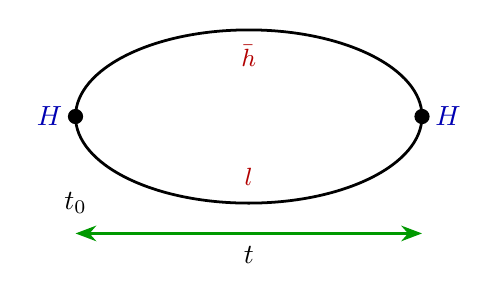
\begin{tikzpicture}[>=Stealth,thick,scale=1.1]
  % Parameters
  \def\R{2}      % horizontal radius
  \def\H{1}    % vertical radius

  % Coordinates
  \coordinate (L) at (-\R,0);  % left source
  \coordinate (R) at ( \R,0);  % right sink

  % Upper arc: R -> L (flowing left)
  \draw[line width=1pt] (R) arc[start angle=0,end angle=180,x radius=\R,y radius=\H];
  % Lower arc: L -> R (flowing right)
  \draw[line width=1pt] (L) arc[start angle=180,end angle=360,x radius=\R,y radius=\H];

  % Endpoints
  \fill (L) circle (2.5pt);
  \fill (R) circle (2.5pt);

  % Current insertion J: at top arc halfway
  \path (R) arc[start angle=0,end angle=100,x radius=\R,y radius=\H] coordinate (J);
  %\fill (J) circle (2.5pt);
  %\node[blue!70!black, font=\bfseries] at ($(J)+(0.2,0.3)$) {$J$};

  % Meson labels
  %\node[blue!70!black, font=\bfseries] at ($(L)+(-0.52,0.0)$) {$H,H_s$};
  %\node[blue!70!black, font=\bfseries] at ($(R)+(0.5,0.0)$) {$\pi,K$};

  \node[blue!70!black, font=\bfseries] at ($(L)+(-0.3,0.0)$) {$H$};
  \node[blue!70!black, font=\bfseries] at ($(R)+(0.3,0.0)$) {$H$};

  % Flavour labels inside loop
  %\node[red!70!black, font=\small] at (-1.2,0.5) {$\bar{l}$};
  \node[red!70!black, font=\small] at ( 0,+0.7) {$\bar{h}$};
  %\node[red!70!black, font=\small] at ( 0,-0.7) {$l,s$};
  \node[red!70!black, font=\small] at ( 0,-0.7) {$l$};

  %mass comparison
  %\node[black!70!black, font=\small] at ($(J)+(2,0.3)$) {$m^\mathrm{phys}_c \leq m_h \leq m^\mathrm{phys}_b$};

  % Green t arrow (horizontal above loop)
  %\draw[green!60!black,<->,line width=1pt] ($(L)+(0,\H+0.2)$) -- ($(J)+(0,\H-0.75)$);
  %\node[black!60!black] at ($(J)+(-0.8,0.45)$) {$t$};
  
  % Green baseline and T arrow (below loop)
  \draw[green!60!black,<->,line width=1pt] ($(L)+(0,-\H-0.35)$) -- ($(R)+(0,-\H-0.35)$);
  \node[black!60!black] at ($(L)+(0,-\H)$) {$t_0$};
  \node[black!60!black] at ($(0,-\H*1.6)$) {$t$};
  
\end{tikzpicture}

\end{document}